%% ------------------------------------------------------------------------- %%
\chapter{Methods, Results, and Conclusions}
\label{cap:conclusoes}

\section{Methods}

Matrix norms were used to assert the correctness of our results. 
Let %$x \in \Cfield^n$ and 
$A \in \Cfield^{m \times n}$. \cite{watkins:2004} defines  
matrix 1-norm as:
\begin{equation}
%	\norm{x}_{\infty} = \max\limits_{1 \leq k \leq n} |x_k| \qquad 
%	\norm{A}_{\infty} = \max\limits_{1 \leq i \leq m} \sum_{j=1}^{n} |a_{ij}| \quad
	\norm{A}_{   1  } = \max\limits_{1 \leq j \leq n} \sum_{i=1}^{m} |a_{ij}| \quad
\end{equation}

All norms have the property that $\norm{A} = 0$ if and only if $A = 0$.
Let $u$ and $v$ be two numerical 
algorithms that solve the same problem, but in a different way. 
Now let $y_u$ be the result computed by $u$ and $y_v$ be the result computed by
$v$. The \textit{error} between these two values can be measured computing
$\norm{y_u - y_v}$. The error between CPU and GPU versions of $H$ and $G$ matrices was computed by calculating $\norm{H_{cpu} - H_{gpu}}_1$
and $\norm{G_{cpu} - G_{gpu}}_1$. An automated test check if this value is bellow $10^{-4}$.

Gfortran and CUDA 8.0 were used to compile the application. The main flags used in Gfortran were
$\texttt{-Ofast}$ $\texttt{-march=native}$ $\texttt{-funroll-loops}$ $\texttt{-flto}$. The flags used in
CUDA nvcc compiler were: $\texttt{-use\_fast\_math}$  $\texttt{-O3}$ $\texttt{-Xptxas}$ $\texttt{--opt-level=3}$
$\texttt{-maxrregcount=32}$ $\texttt{-Xptxas}$ 
$\texttt{--allow-expensive-optimizations=true}$ . 

For experimenting, there were four data samples as shown in Table \ref{experiments}. Each routine defines 
the label \texttt{gpu} in its context, but the \texttt{cpu} label means that the routine was executed only in CPU. 

Before any data collection, a warm up procedure is executed, which consists of running the 
application with the sample three times without getting any result. Afterward, all experiments 
were executed 30 times per sample. Each execution produced a file with total time elapsed, 
where a script computed averages and standard deviations for all experiments.

The graphs labels consist of the implementation name concatenated with the number of OpenMP threads used, 
for example, \texttt{cpu8} implies that only the CPU was used with 8 OpenMP threads. All its points 
are the mean of the time in seconds of 30 executions, and the errorbars illustrate a 95\% confidence interval.

The number of threads used were defined considerating the number of CPU cores the testing machine has. 
We used two machines for the tests, \texttt{BrucutuIV} and \texttt{Venus}, as defined in Appendix $\ref{cap:ape}$

GPU total time was computed by the sum of 5 elements: 
(1) total time to move data to GPU, (2) launch and execute the kernel, (3) elapsed time 
to compute the result, (4) time to move data back to main memory, (5) time to compute 
any remaining parts in the CPU. 
The elapsed time was computed in seconds with the OpenMP library function 
$\texttt{OMP\_GET\_WTIME}$. This function calculates the elapsed wall clock time in seconds 
with double precision. All experiments set the Gauss Quadrature Points to 8.

\begin{table}[]
\centering
\caption{Data experiment set}
\label{experiments}
\begin{tabular}{|l|l|l|l|l|l|}
\hline
Number of Mesh elements     & 240 & 960 & 2160 & 4000 & 14400\\ \hline
Number of Boundary elements & 100 & 400 & 900  & 1600 & 6400\\ \hline
\end{tabular}
\end{table}

\section{Results}

\subsection{Ghmatecd Routine}

This routine has three parallel implementations: (1) Using only CPU threads 
(\texttt{cpu}); (2) Using GPU for the nonsingular part and the CPU for the 
singular part, as described by Algorithm $\ref{ghmatecd_new}$ (\texttt{gpu}); 
(3) Using GPU for both singular and nonsingular parts, as described by Algorithm 
$\ref{ghmatecd_new2}$ (\texttt{gpu\_sing}).                                    

\subsubsection{BrucutuIV Data}

The logarithmic scale graphic at Figure $\ref{fig:ghmatecd_brucutuiv_non_sequential}$ illustrates the
results for \texttt{BrucutuIV}. We removed the points from the graph that represents the sequential data for legibility.

\begin{figure}[ht]
\centering
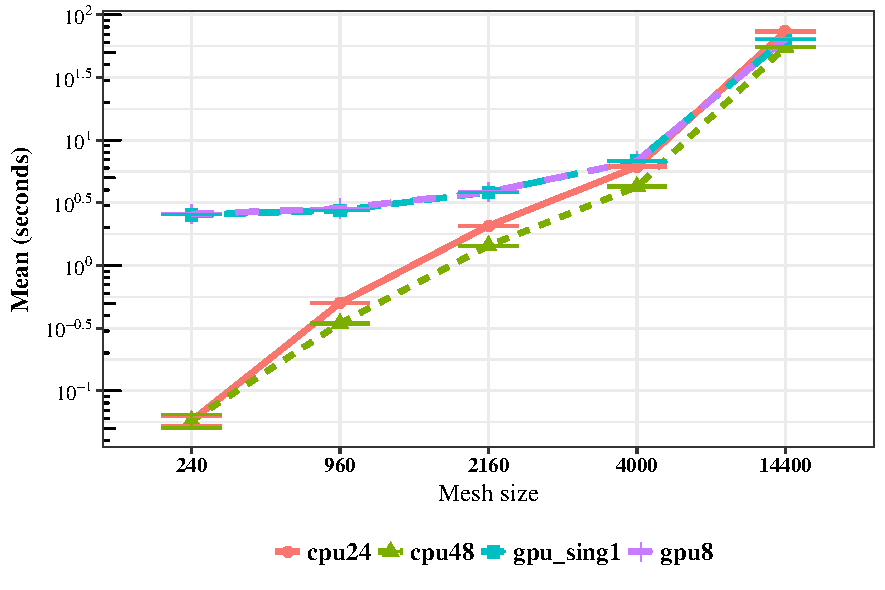
\includegraphics[scale=1]{ghmatecd_brucutuiv_non_sequential.pdf}
\caption{GHMATECD: Time elapsed by each implementation in logarithm scale}
\label{fig:ghmatecd_brucutuiv_non_sequential}
\end{figure}

The speedup acquired in the $14400$ mesh elements sample with \texttt{cpu48}, \texttt{cpu24} 
\texttt{gpu8} and \texttt{gpu\_sing1} with respect to the sequential algorithm are 
$25$, $19$, $22$ and $22$ respectively in \texttt{BrucutuIV}. For this sample we can see that a single Tesla K40
was faster than a single Xeon E5-2650 v4, but slower than two of those processors.

Notice that with respect to time, \texttt{gpu8} and \texttt{cpu\_sing1} behaves very similarly, 
but there is an interesting observation about the error, as illustrated by 
Figure $\ref{fig:ghmatecd_brucutuiv_error}$. 

\begin{figure}[ht]
\centering
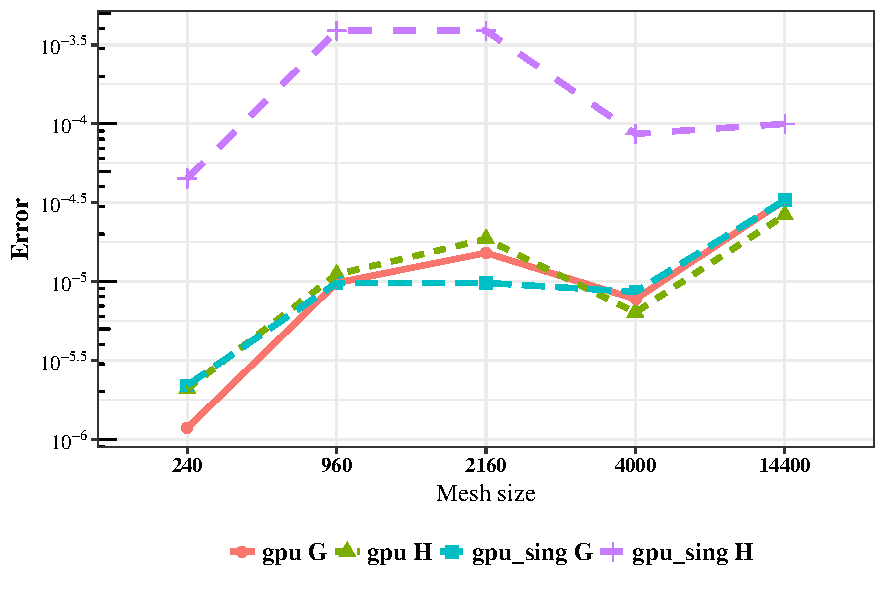
\includegraphics[scale=1]{ghmatecd_brucutuiv_error.pdf}
\caption{GHMATECD: Error of each implementation compared with the CPU implementation}
\label{fig:ghmatecd_brucutuiv_error}
\end{figure}

Since there is an error gap in the $H$ matrix between the \texttt{gpu8} and \texttt{gpu\_sing1}, it suggests that most 
errors concentrate arround computation of the singular case and it is more sensible to floating point erros, thus better 
precision is required here.

As a conclusion, the presented method can be used to accelerate the overall performance of the mentioned routine, 
and a load balancer can be developed from these results for even higher speedups because of two items: (1) similar 
computational time elapsed between \texttt{gpu\_sing1} and \texttt{cpu24} in the $14400$ sample, and (2) 
the fact that \texttt{gpu\_sing1} only uses one CPU thread, allowing other threads to also consume workload.

\subsubsection{Venus Data}

Here the obtained speedup was $3$, $100$ and $100$ respectively for the \texttt{cpu4}, 
\texttt{gpu4} and \texttt{gpu\_sing1} on the $4000$ mesh sample. We could not run the $14400$ 
sample because it requires around $16$ Gigabytes of RAM, but the machine only had $8$ Gigabytes.
Notice that the GeForce GTX980 was faster than the AMD A10-7700K even for the 960 sample. This was due to 
lower CPU-GPU memory transfer latency. The logarithm graphic at 
Figure $\ref{fig:ghmatecd_venus_1}$ illustrates the results.

\begin{figure}[ht]
\centering
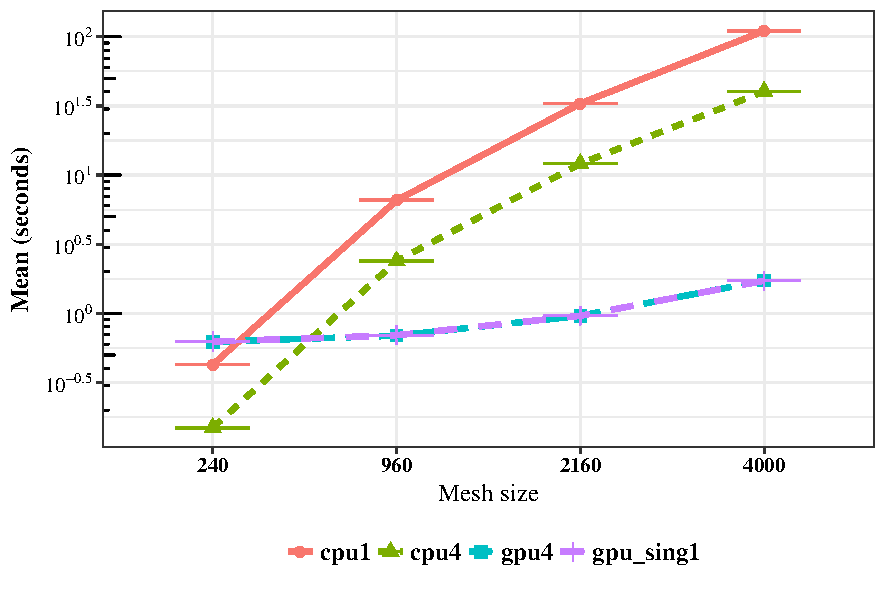
\includegraphics[scale=1]{ghmatecd_venus_1.pdf}
\caption{Time elapsed by each implementation in logarithm scale}
\label{fig:ghmatecd_venus_1}
\end{figure}

The errors followed the same behavior as discussed in \texttt{BrucutuIV Data} section, as illustrated in 
Figure $\ref{fig:ghmatecd_venus_error}$. Notice that the errors in $H$ are worse when compared to
\texttt{BrucutuIV}.

\begin{figure}[ht]
\centering
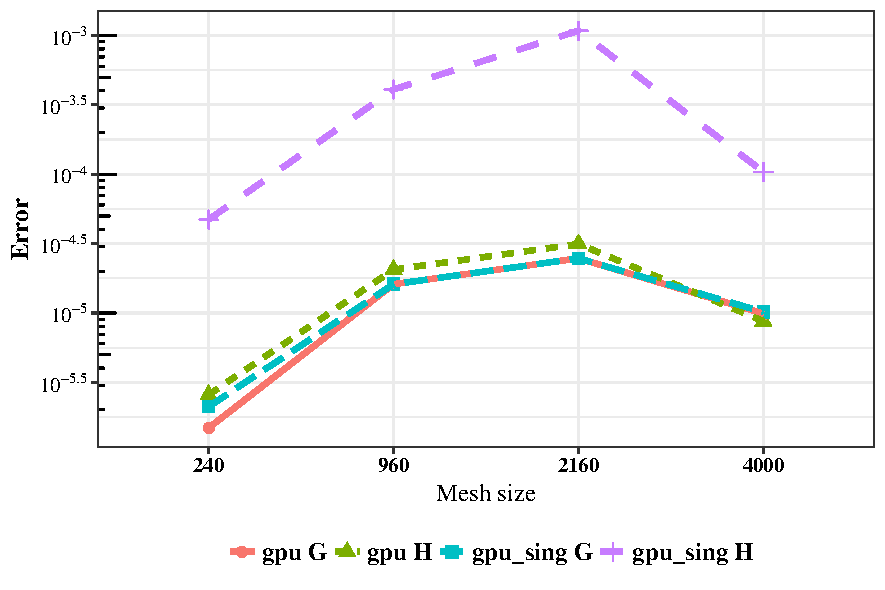
\includegraphics[scale=1]{ghmatecd_venus_error.pdf}
\caption{GHMATECD: Error of each implementation compared with the CPU implementation}
\label{fig:ghmatecd_venus_error}
\end{figure}

From these data, we can conclude that the presented method can also accelerate the performance in 
the case that there is a low number of CPU cores available, and such CPU cores can be allocated to 
compute the singular case to reduce errors. 

\subsection{Ghmatece Routine}

This routine has two parallel implementations: (1) Using only CPU threads (\texttt{cpu}); 
(2) Using GPU for the nonsingular part and the CPU for the singular part (\texttt{gpu}), 
as presented by the technique in Algorithm $\ref{ghmatecd_new}$. 

\subsubsection{BrucutuIV Data}

The logarithm graphic in Figure $\ref{fig:ghmatece_brucutuiv_1}$ illustrates the results.
The speedup acquired in the 14400 mesh elements sample with \texttt{cpu24}, \texttt{cpu48}, and \texttt{gpu8} 
with respect to the sequential algorithm are 15, 19, and 13 respectively in \texttt{BrucutuIV}. For this sample, 
we can see that the Tesla K40 was slower than a single Xeon E5-2650 v4. Although \texttt{Ghmatece} routine is similar 
to \texttt{Ghmatecd}, it does fewer computations and thus the usage of GPUs here may not be attractive here.

\begin{figure}[ht]
\centering
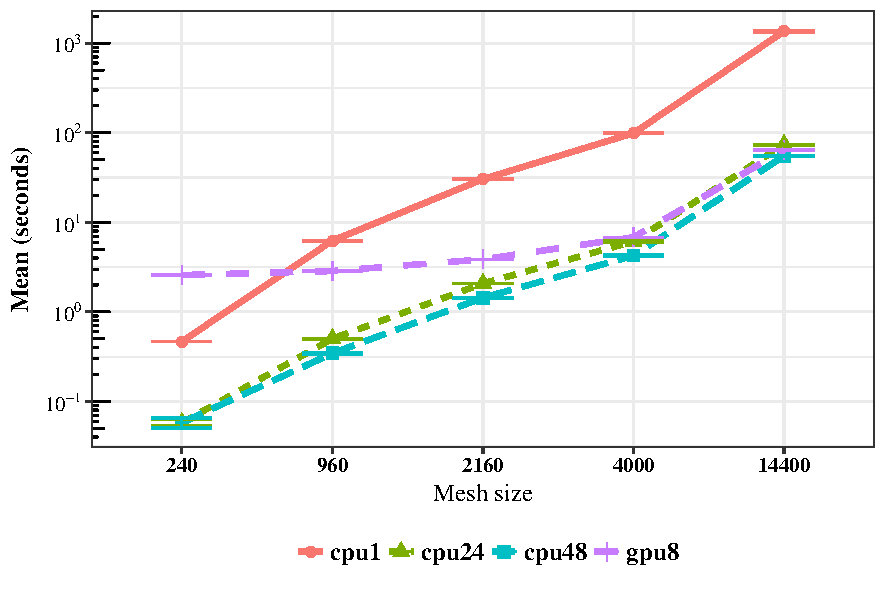
\includegraphics[scale=1]{ghmatece_brucutuiv_1.pdf}
\caption{Time elapsed by each implementation in logarithm scale}
\label{fig:ghmatece_brucutuiv_1}
\end{figure}


As for the error, the $14400$ was the only sample that had errors bigger than $10^{-5}$. Since the $||\bullet||_1$
grows as the number of matrix rows increases, this result was expected. Figure $\ref{fig:ghmatece_brucutuiv_error}$
illustrates the results.

\begin{figure}[ht]
\centering
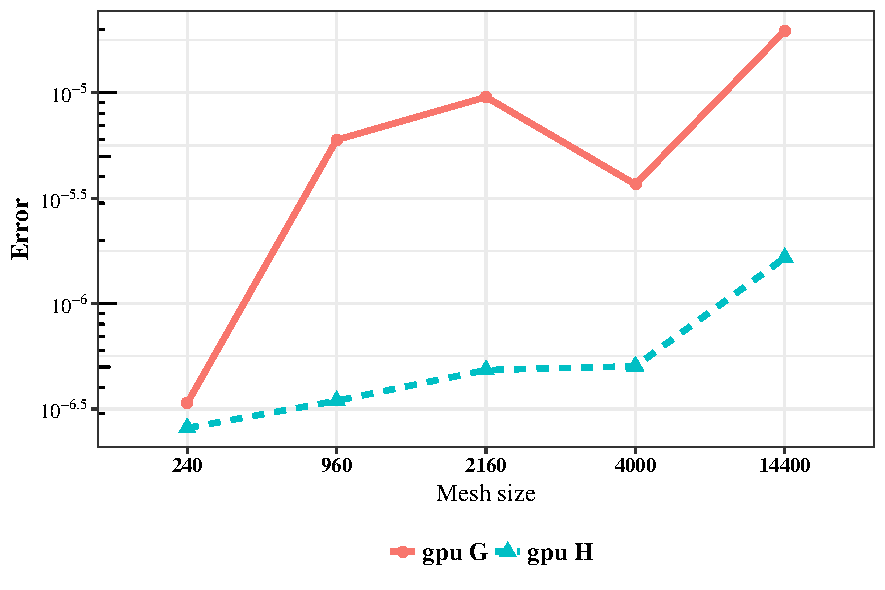
\includegraphics[scale=1]{ghmatece_brucutuiv_error.pdf}
\caption{GHMATECE: Error of each implementation compared with the CPU implementation}
\label{fig:ghmatece_brucutuiv_error}
\end{figure}
